%************************************************
%\section{Appendix}
%\label{sec:appendix}
%************************************************
\begin{appendix}

\section{SRSCT}
\label{sec:srsct}

\subsection{SRSCT experiment}
\label{subsec:srsctexperiment}
A representative sample of bulk solid was placed in a shear cell of specified dimensions ($external ~ radius = 100 ~ mm$, $internal ~ radius = 50 ~ mm$). 
\begin{figure}[!htb] 
\centering 
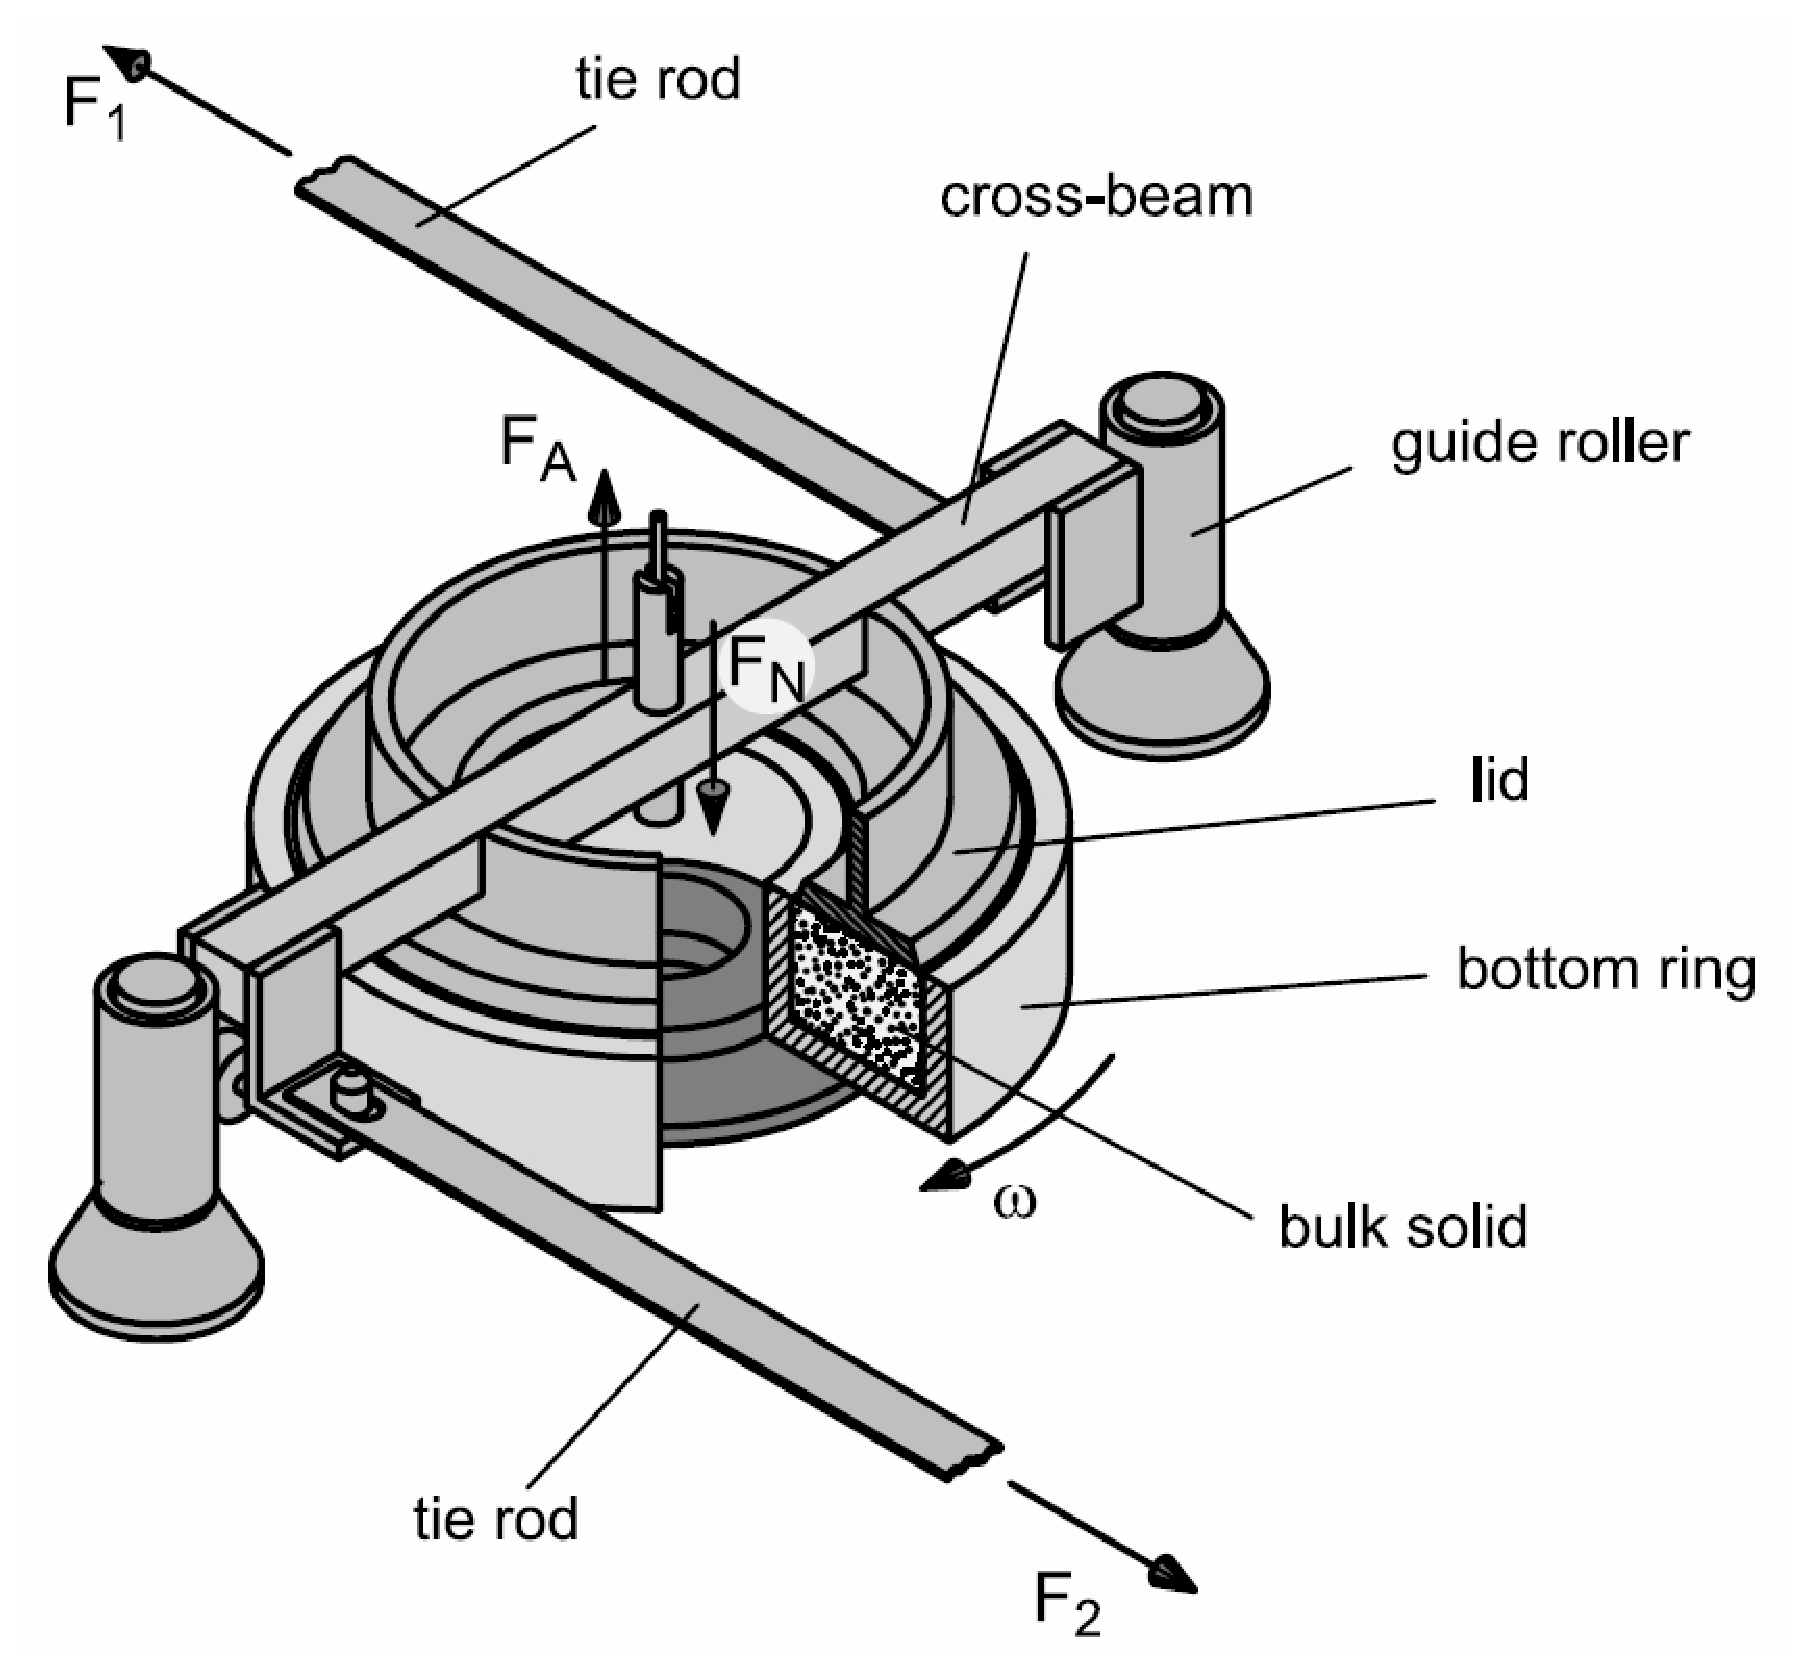
\includegraphics[width=.8\textwidth]{images/original/01srsct} 
\caption[Schulze ring shear cell tester]{Schulze ring shear cell tester
experimental layout, Schulze \cite{RefWorks:118}}
\label{fig:01srsct} 
\end{figure}


% \begin{figure}[htp]
%     \centering
%     
\includegraphics[width=.2\textwidth]{images/vitae/lbenvenuti}
%     \caption{OpenMP, MPI, MPI/OpenMP Hybrid runs of Box in a box testcase on 32
%     cores. The OpenMP-only run suffers from limited memory bandwidth in
%     memory-bound algorithms inside of the Modify section of the code. MPI-only has
%     low averaged runtimes for each section, but a very large Other timing, which
%     hints for a large amount of load-imbalance. Hybrid timings are a bit worse
%     on average, but because of better balancing, processes have lower wait times
%     inside of Other timing.}
% 	\label{fig:boxInBoxComparison}

A normal load was applied to the cover. As soon as the lid touches the sample, its position is calculated. Together with the area of the ring, the total volume can be calculated, and subsequently the $bulk ~ density ~ (\rho_b)$ of the sample is obtained, the first value representative of the bulk behaviour. Then the specimen was pre-sheared until a steady-state shear value was reached. The steady-state flow horizontal stress (Fig. \ref{fig:02srsctdiagram}) is called $steady-state-flow/pre-shear$ stress ($\tau_{psh}$). Knowing the normal stress, it gives (Eq. \ref{eq:phi_ps}) the angle of internal friction of the pre-shear phase ($\phi_{e-psh}$), and consequently the $coefficient-of-internal-friction $ $ (\mu_{psh})$, the second behaviour value. \cite{RefWorks:118}:


\begin{equation}
\begin{aligned}
\phi_{e-psh} &= \arctan \left(\frac{\tau_{psh}}{\sigma_{n,psh}} \right) ,\\
\mu_{psh} &=\tan(\phi_{e-psh}) .
\end{aligned}
 \label{eq:phi_ps}
\end{equation}
   
\begin{figure}[!htb] 
\centering 
\includegraphics[width=.8\textwidth]{images/original/02srsctdiagram.eps} 
\caption{Schulze ring shear cell tester diagram \cite{RefWorks:118}}
\label{fig:02srsctdiagram} 
\end{figure}


% \begin{figure}[htp]
%     \centering
%     
\includegraphics[width=.2\textwidth]{images/vitae/lbenvenuti}
%     \caption{OpenMP, MPI, MPI/OpenMP Hybrid runs of Box in a box testcase on 32
%     cores. The OpenMP-only run suffers from limited memory bandwidth in
%     memory-bound algorithms inside of the Modify section of the code. MPI-only has
%     low averaged runtimes for each section, but a very large Other timing, which
%     hints for a large amount of load-imbalance. Hybrid timings are a bit worse
%     on average, but because of better balancing, processes have lower wait times
%     inside of Other timing.}
% 	\label{fig:boxInBoxComparison}

The normal stress and the angular velocity were then immediately reduced to zero. 
Subsequently, the specimen was sheared under a fraction ($shear-perc$) of the first normal load until the shear force reached a maximum and began to decrease. 
Both the pre-shear and shear phases were executed at constant velocity. We define the horizontal stress during the shear force peak as maximum shear stress, thus obtaining $incipient-flow/shear ~ coefficient-of-internal-friction $ $ (\mu_{sh})$, third behaviour value (Eq. \ref{eq:phi_s})\cite{RefWorks:118}:


\begin{equation}
\begin{aligned}
\phi_{e-sh} &= \arctan \left(\frac{\tau_{sh}}{\sigma_{n,sh}} \right) ,\\
\mu_{sh} &= \tan(\phi_{e-sh}) .
\end{aligned}
 \label{eq:phi_s}
\end{equation}
 
From two to three different pre-shear normal loads were applied in the experiment. For each we used a normal load proportional to the initial one ($shear-perc$) increasing from stage one (40\%) to stage four (100\%) with two escalating intermediate stages (60\% and 80\%).
Each experiment was performed on a fresh material sample. \\

\subsection{SRSCT simulation}
\label{subsec:srsctsimulation}
$LIGGGHTS$, the simulation toolbox we used, meets all the requirements of modelling the shear tester described in the appendix A1. First, it is capable of importing triangulated meshes of the two rings and a top lid. Since the real set-up had a wall thickness, contact forces acting on a mesh are summed and can be saved, and thus shear force calculation is available out of the box. Moreover, the code can move a mesh with constant velocity as required for the measurement. To determine the shear stresses, the bulk solid had to be stressed with user-defined normal stresses. Therefore, a stress-controlled wall ($servo-wall$ in $LIGGGHTS$) was applied to the lid. \\
Although the geometry differs, the $SRSCT$ was designed to obtain the same values for the shear stresses as the Jenike shear cell tester ($JSCT$), but with improved automation and reliability \cite{RefWorks:118}. For this reason, the simulation setup has been based over the $JSCT$. The layout of the simulation geometry can be seen in Figure \ref{fig:09simGeometry}. As suggested by Aigner et al. \cite{RefWorks:139} and Benvenuti et al. \cite{RefWorks:173}, the diameter and the height of the rings operated in the simulations had to be sufficiently large to avoid relevant wall effects. Nevertheless, a larger domain increases the number of particles, and thus the simulation time. For this reason, we considered the cylinders dimension, as proportion to the mean particle diameter ($dCylDp$), an additional DEM parameter investigated. \\   \begin{figure}[!htb] 
\centering 
\includegraphics[width=.8\textwidth]{images/original/09simGeometry} 
\caption{shear cell simulation layout}
\label{fig:09simGeometry} 
\end{figure}


% \begin{figure}[htp]
%     \centering
%     
\includegraphics[width=.2\textwidth]{images/vitae/lbenvenuti}
%     \caption{OpenMP, MPI, MPI/OpenMP Hybrid runs of Box in a box testcase on 32
%     cores. The OpenMP-only run suffers from limited memory bandwidth in
%     memory-bound algorithms inside of the Modify section of the code. MPI-only has
%     low averaged runtimes for each section, but a very large Other timing, which
%     hints for a large amount of load-imbalance. Hybrid timings are a bit worse
%     on average, but because of better balancing, processes have lower wait times
%     inside of Other timing.}
% 	\label{fig:boxInBoxComparison}
 
A simulation run comprised four phases. First, the shear cell was filled with the granulate material, and it was allowed to settle. Then, the top lid was lowered and applied the first normal stress to the bulk solid. As in the experiment, the servo-wall allows to calculate the position of the lid while the first particle is touched. Together with the simulation area, we calculated $\rho_b$. Next, the ring moved for a distance $l=0.1875 \cdot radius ~of ~the ~ring$, and the required pre-shear force was measured. Finally, the normal load was reduced to a fraction of the initial load, the ring was moved again by a distance $l$, and the shear force was recorded. Unlike in the original experiment, the bottom ring was moved to facilitate the numerical simulation. The velocity of the ring displacement, and consequently the total simulation time, are determined through a challenging equilibrium between the downgrading of normal load oscillation and the computational time containment. The former is obtained by low (relatively) velocity, the latter by high speed. We imposed a constant velocity of $3*(mean particle radius)/seconds$, the most suitable to satisfy the two competing requests. \\
The normal stresses (pre-shear and shear phases) applied in each simulation were the same as in the experiments. The corresponding $\tau_{psh}$ and $\tau_{sh}$ were calculated - as in the experiments - from the mean of the plateau.\\

\section{AOR}
\label{sec:AOR}

\subsection{AOR experiment}
\label{subsec:aorexperiment}
A sample was deposited on a 20 cm diameter plate with lift-able boundary, called static angle of repose ($AOR$) tester (Fig. \ref{fig:05aor}).
\begin{figure}[!htb] 
\centering 
\includegraphics[width=.8\textwidth]{images/original/05aor} 
\caption[Angle of repose tester]{Angle of repose tester, Schulze
\cite{RefWorks:118}}
\label{fig:05aor} 
\end{figure}


% \begin{figure}[htp]
%     \centering
%     
\includegraphics[width=.2\textwidth]{images/vitae/lbenvenuti}
%     \caption{OpenMP, MPI, MPI/OpenMP Hybrid runs of Box in a box testcase on 32
%     cores. The OpenMP-only run suffers from limited memory bandwidth in
%     memory-bound algorithms inside of the Modify section of the code. MPI-only has
%     low averaged runtimes for each section, but a very large Other timing, which
%     hints for a large amount of load-imbalance. Hybrid timings are a bit worse
%     on average, but because of better balancing, processes have lower wait times
%     inside of Other timing.}
% 	\label{fig:boxInBoxComparison}

Once the particles were in position, the boundary was lifted, allowing some particles to drop. Once stabilized, the $AOR$ was measured eight times using a digital protractor at different positions of the heap. The result is given as the average of the measurements, granting the fourth behaviour value.
Notably, the experiments were performed only for larger size bulk solids. So, the compaction condition in the initial state was not critical to the final result.

\subsection{AOR simulation}
\label{subsec:aorsimulation}
In $AOR$ simulations we tried to replicate meticulously the experimental set-up, considering both the plate and the lift-able boundary, with the same domain size consideration as before. The particles had the same properties as in the shear cell simulation. The first phase was identical to that of the shear cell simulation. 
After lifting the boundary, the particles formed a heap (Fig. \ref{fig:08aorsim}). 
\begin{figure}[!htb] 
\centering 
\includegraphics[width=.8\textwidth]{images/original/08aorsim} 
\caption[AOR simulation]{Angle of repose tester, numerical heap
of particles}
\label{fig:08aorsim} 
\end{figure}


% \begin{figure}[htp]
%     \centering
%     
\includegraphics[width=.2\textwidth]{images/vitae/lbenvenuti}
%     \caption{OpenMP, MPI, MPI/OpenMP Hybrid runs of Box in a box testcase on 32
%     cores. The OpenMP-only run suffers from limited memory bandwidth in
%     memory-bound algorithms inside of the Modify section of the code. MPI-only has
%     low averaged runtimes for each section, but a very large Other timing, which
%     hints for a large amount of load-imbalance. Hybrid timings are a bit worse
%     on average, but because of better balancing, processes have lower wait times
%     inside of Other timing.}
% 	\label{fig:boxInBoxComparison}
 
An image post-processing software was used to obtain the average slope. (NOT TRUE, COMPUTE CROSSSECTION)

\end{appendix}\